Our goal was to build a data-driven taxonomy of bus crashes which classifies accidents into cohesive groups that share recurrent characteristics. The broad class of clustering techniques naturally lends itself to this task, because they are intended to identify emergent group structures from data in an unsupervised way \citep{friedman:elements}.

We adopted the two-stage clustering method of \citet{prato2013bus}, who performed the primary study of bus accident taxonomy. In the first stage, we reduced the dimensionality of the data using self-organizing maps (SOM) \citep{kohonen1982}. A SOM is an artificial neural network that reduces a high-dimensional input space to a low-dimensional, topographic map of the input space. Frequently, a two-dimensional map is used which consists of a grid of neurons. The SOM algorithm maps high-dimensional observations to the lower-dimensional plane, and organizes the neurons spatially. The method is structured so each neuron represents a unique region of the input space, and the overall grid of neurons covers the entire input space.

%Figure \ref{fig:som} provides an illustration of the training process for the SOM algorithm. The SOM algorithm can thus be viewed as a clustering algorithm is its own right, with each neuron representing a cluster of observations. \par

%\begin{figure}[t]
%        \includegraphics[scale=0.3]{som.png}
%        \centering
%        \caption{An illustration of the training of a self-organizing map. The blue blob is the distribution of the training data, and the small white disc is the current training datum drawn from that distribution. At first (left) the SOM nodes are arbitrarily positioned in the data space. The node (highlighted in yellow) which is nearest to the training datum is selected. It is moved towards the training datum, as (to a lesser extent) are its neighbors on the grid. After many iterations the grid tends to approximate the data distribution (right). \citep{wiki:som}}
%        \label{fig:som}
%\end{figure}

To organize the neurons, the SOM algorithm utilizes competitive learning, in which neurons compete among each other to represent input data vectors. Associated with each neuron is a weight vector with the same dimension as the input vectors. When the SOM considers a randomly-selected input vector, the neuron whose weight vector is ``closest'' to the input vector is deemed the winner. This nearest neuron is called the best matching unit (BMU). Then, the weights of the BMU and the neurons close to it in the SOM grid are adjusted towards the input vector. This procedure is repeated until convergence, at which point the neurons cease to ``move''---that is, their weight vectors do not change \citep{kohonen1990}. \par
%%%%%%%%%%%%%%%%%%%%%%%%%%%%%%%%%%%%%%%%%%%%%%%%%%%%%%%%%%%%%%%%%%%%%%%%%%%%%%%%%%%%
\begin{figure}[t]
        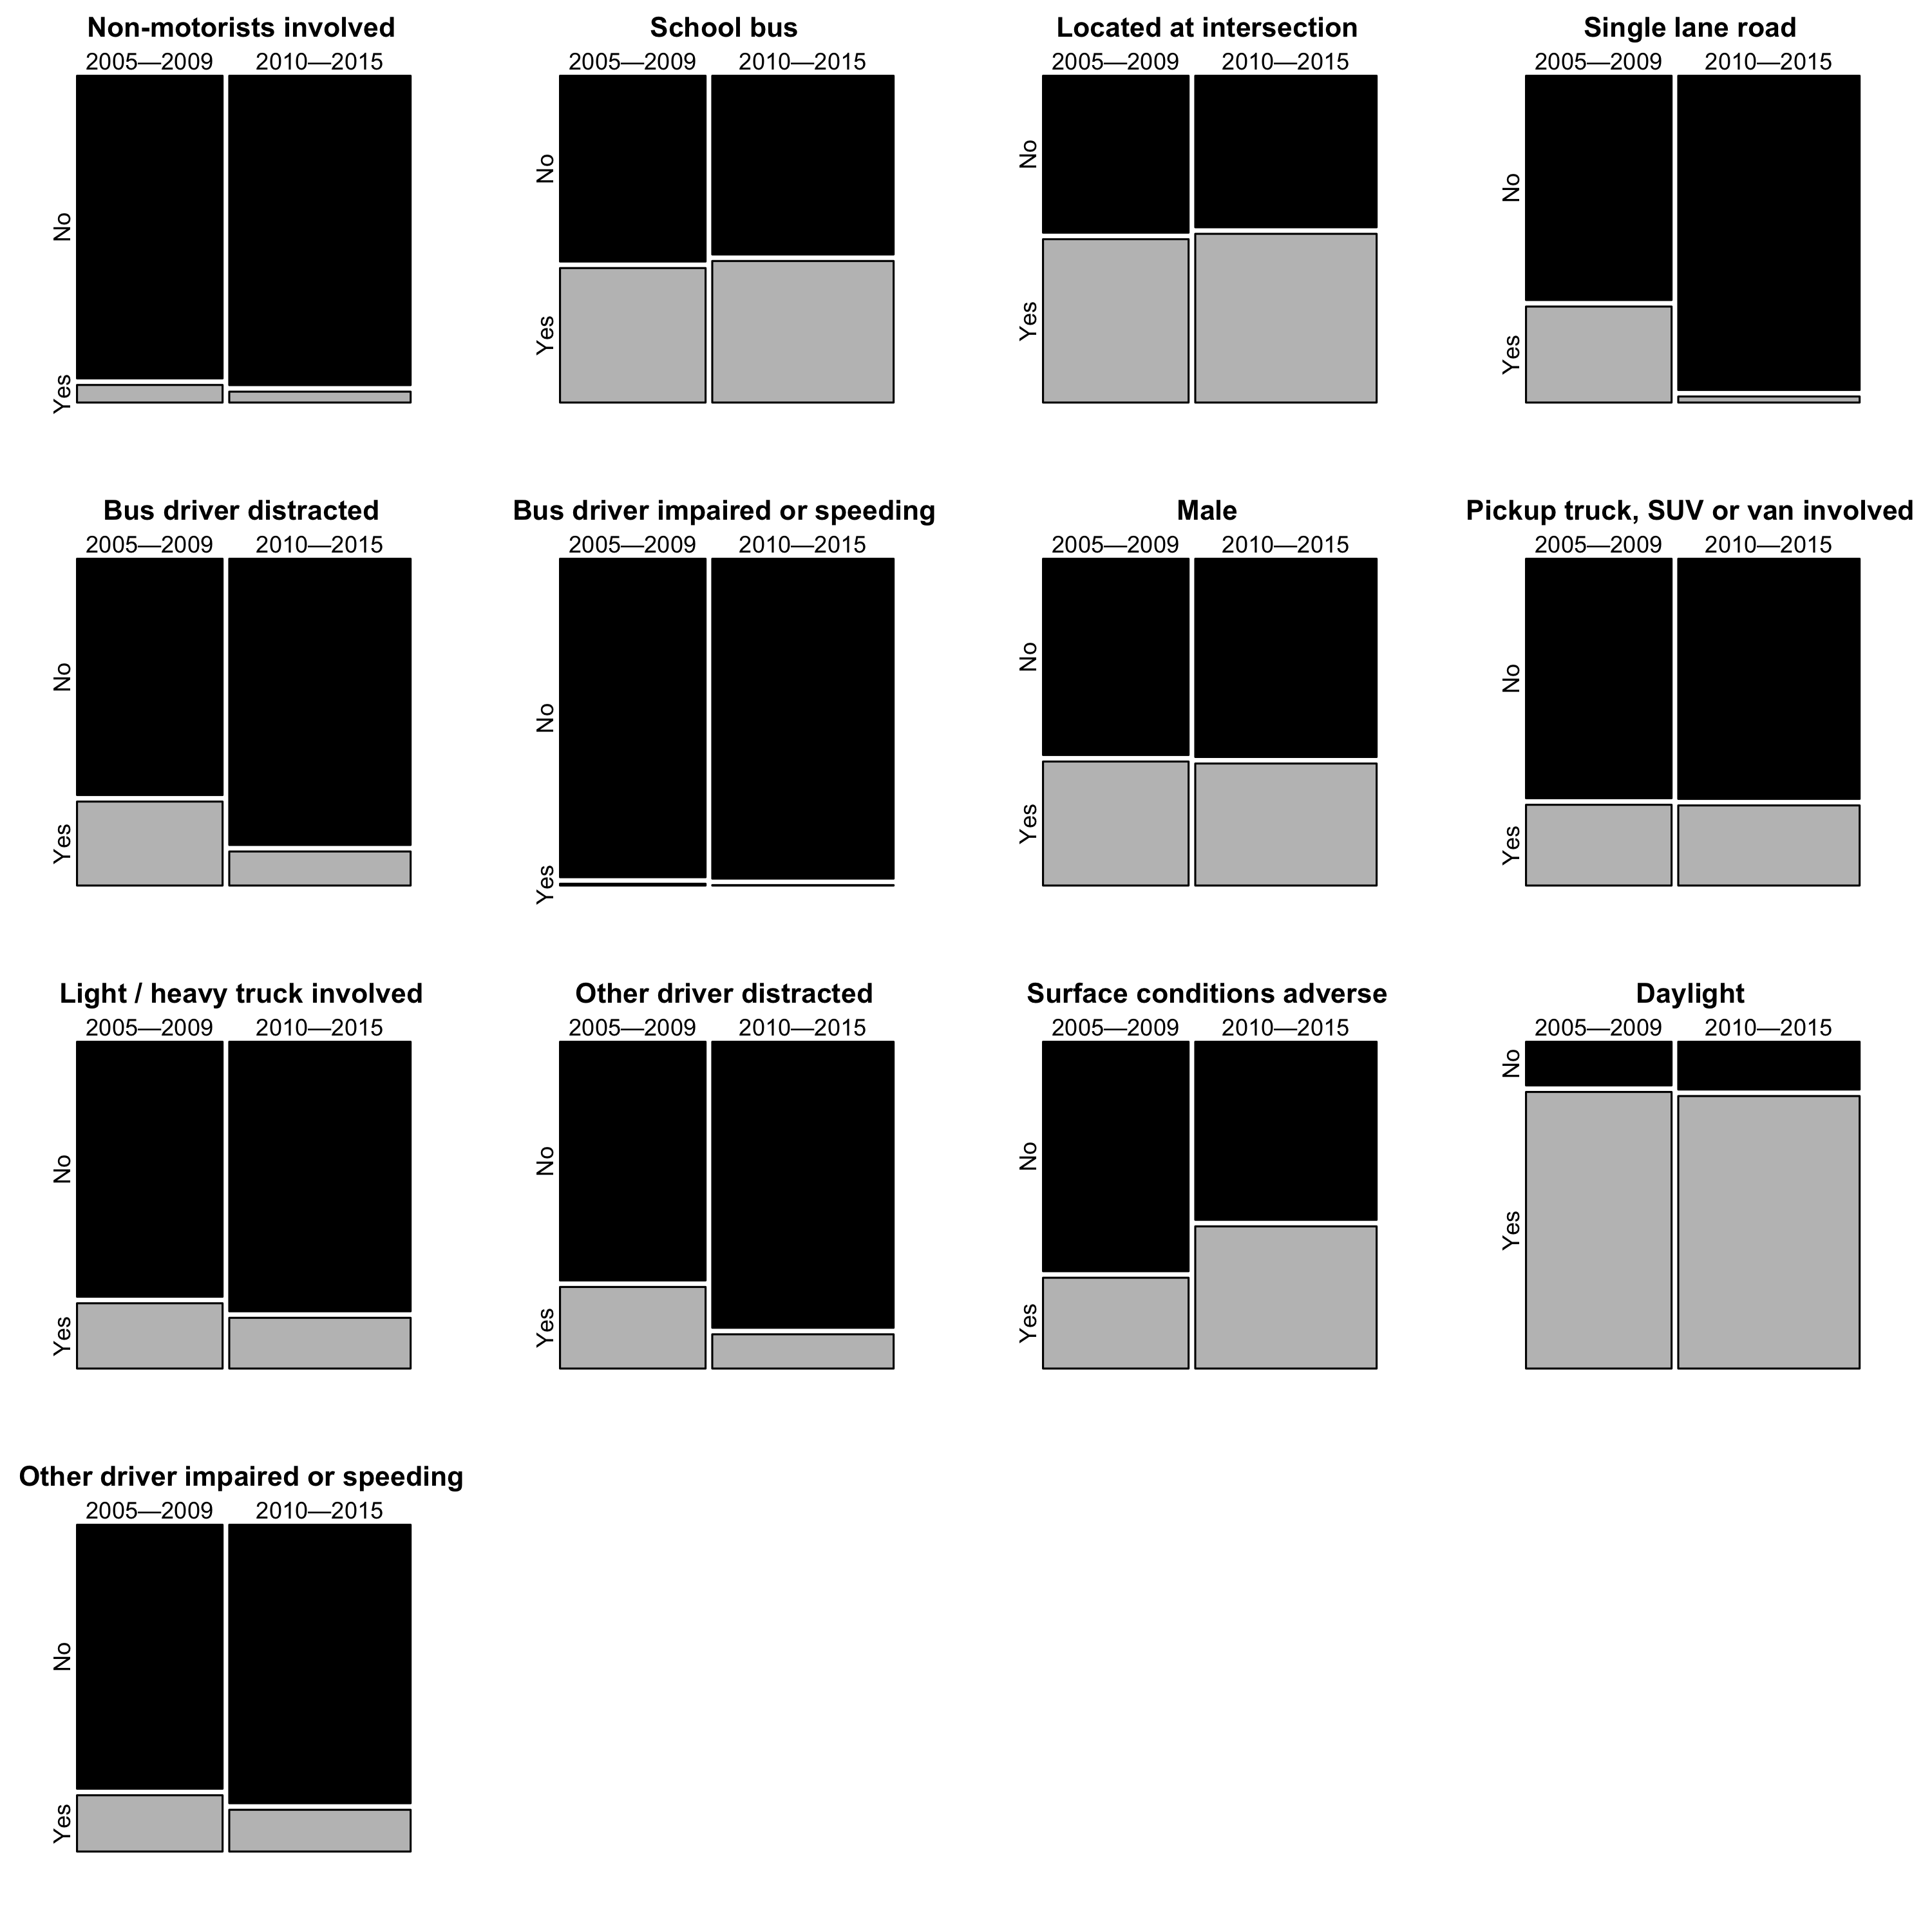
\includegraphics[width=\textwidth]{props.png}
                \caption{Mosaic plots comparing the binary response variables across the 2005--2009 
                and 2010--2015 datasets}
        \label{fig:props1}
\end{figure}
%%%%%%%%%%%%%%%%%%%%%%%%%%%%%%%%%%%%%%%%%%%%%%%%%%%%%%%%%%%%%%%%%%%%%%%%%%%%%%%%%%%%
In the second stage of clustering, we applied the neural gas algorithm of \citet{martinetz1991} to the self-organizing map from the first stage, thereby producing the final clustering.
The neural-gas clustering algorithm was historically inspired by the SOM algorithm and can be viewed a robust version of the sequential $K$-means algorithm \citep{macqueen1967}. In sequential $K$-means, cluster centers are updated by processing individual input vector sequentially. This contrasts with the approach of the traditional $K$-means algorithm, which considers all input vectors simultaneously. In the sequential method, only the cluster center closest to the input vector is adjusted towards it. The neural gas algorithm deviates from this by updating \emph{all} the cluster centers at each new input vector, with centers closer to the input vector adjusting more than those far away. This modification provides robustness to noisy input vectors and stabilizes the algorithm's convergence. \par

As mentioned previously, the SOM algorithm is a clustering algorithm in its own right, and hence could be used to form the taxonomy of bus crashes by itself. However, as mentioned in \citet{prato2013bus}, the neural-gas algorithm has advantages over methods like SOM in terms of convergence speed and accuracy \citep{vesanto2000}. The high computational complexity of the neural-gas algorithm, its main disadvantage, is mitigated by its application to the lower-dimensional SOM neuron grid. This allows more flexibility in dealing with high-dimensional output, without sacrificing the practicality of applying the technique. \par
%%%%%%%%%%%%%%%%%%%%%%%%%%%%%%%%%%%%%%%%%%%%%%%%%%%%%%%%%%%%%%%%%%%%%%%%%%%%%%%%%%%%
\begin{figure}[t]
        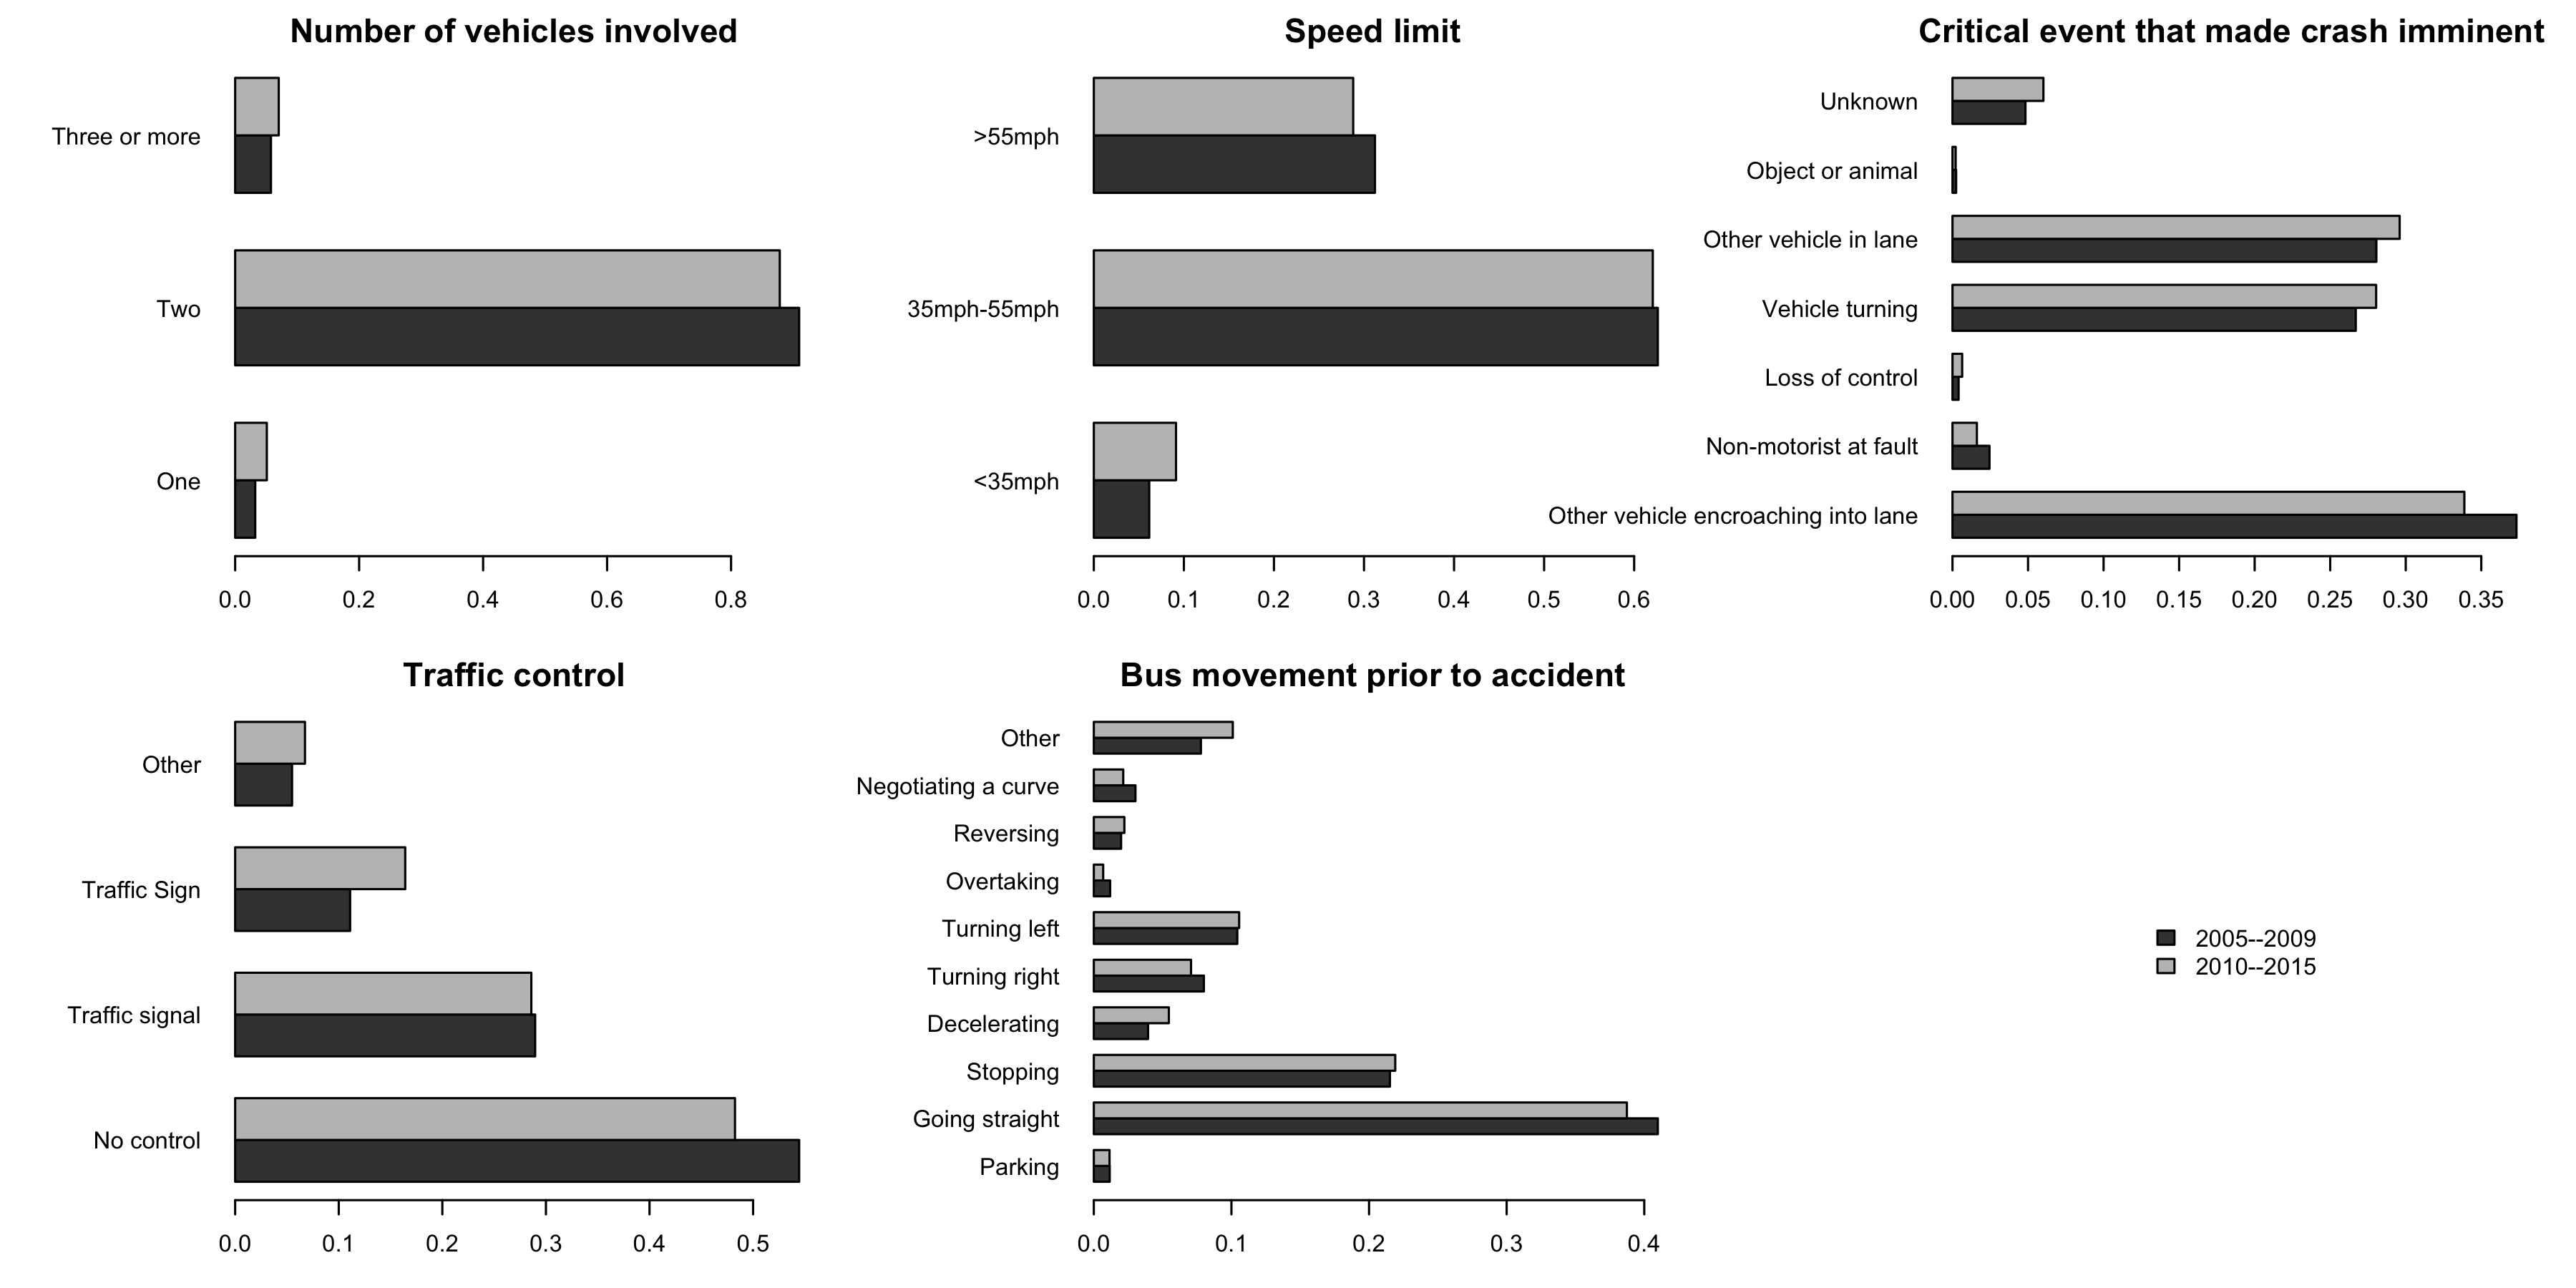
\includegraphics[width=\textwidth]{radar-bar.png}
                \caption{Grouped bar plots comparing the categorical response variables across the 2005--2009 and 2010--2015 datasets.}
        \label{fig:cat1}
\end{figure}
%%%%%%%%%%%%%%%%%%%%%%%%%%%%%%%%%%%%%%%%%%%%%%%%%%%%%%%%%%%%%%%%%%%%%%%%%%%%%%%%%%%%
